%Start
%required packages and reason
\documentclass[11pt]{article}
\usepackage[a4paper,margin=1in]{geometry}
\usepackage{mathtools} % required for sigma notation
\usepackage{graphicx} %required to load images
\usepackage{amsmath} %required for the matrices
\usepackage{upgreek} %required for Greek symbols
\usepackage{xfrac} %for differentiation symbol
\usepackage{float} %to set the figures exactly where we want,(\figure "[H]")
\usepackage{listings} %to get colorful code in latex
\usepackage{color} %to get a nice color scheme
\usepackage{pythonhighlight} %to make the the python codes nice

%initial headings
\title{EE2703 Assignment 6: The Laplace Transform}
\author{Anvith Pabba EE19B070}
\date{20th April 2021}

%begin document
\begin{document}

\maketitle

\section{Introduction}
In this assignment, we look at how to analyse “Linear Time-invariant Systems” using the scipy.signal library in Python.
\\We analyse the outputs of 3 systems:
\begin{enumerate}
    \item A forced spring (oscillatory system)
    \item Coupled system of differential equations
    \item An RLC low pass filter
\end{enumerate}

\section{The Assignment}
\subsection{Question 1 : Response of a spring system}

the time response of the string satisfies
\begin{equation}
    \"{x} + 2.25x = f(t)
\end{equation}

where, the function f(t) is given by:
\begin{equation}
    f(t) = cos(1.5t)exp^{-0.5t}u(t)
\end{equation}

The Laplace transform of f(t), i.e F(s) is given by:
\begin{equation}
    F(s) = \frac{s+0.5}{(s+0.5)^2+2.25}
\end{equation}

On solving the equations in Laplace domain, we get:
\begin{equation}
    X(s) = \frac{s+0.5}{((s+0.5)^2+2.25)(s^2+2.25)}
\end{equation}
We then use impulse response of X(s) to get x(t),

\subsubsection{Plot of x(t)}

\begin{figure}[H]
    \centering
    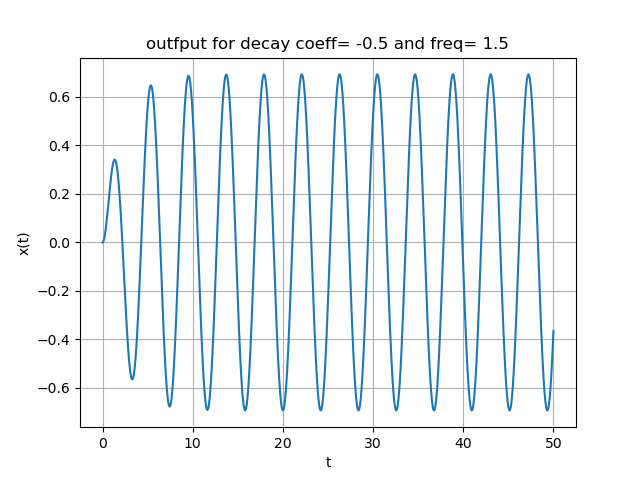
\includegraphics[scale = 1]{Figure_1.png}
    \caption{Response of a forced oscillatory system}
\end{figure}

\subsubsection{Code}
I defined a function that returns the output based on input decay coefficient and frequency.
\begin{python}
def H_s(a,b): #defining the Laplace transform, -a is the decay coefficiant, and b is the frequency
	num = poly1d([1,a])
	den1 = poly1d([1,2*a,a*a + b*b])
	den2 = poly1d([1,0,2.25])
	den = polymul(den1,den2)
	H = sp.lti(num,den)
	return H

H1 = H_s(0.5,1.5)

t,x = sp.impulse(H1,None, linspace(0,50,10000))
plot(t,x)
xlabel('t')
ylabel('x(t)')
title('outfput for decay coeff= -0.5 and freq= 1.5')
grid()
show()

\end{python}

\subsection{Question 2}
now, we find the response for a system given by:
\begin{equation}
    f(t) = cos(1.5t)exp^{-0.05t}u(t)
\end{equation}
In Laplace domain,
\begin{equation}
    F(s) = \frac{s+0.05}{(s+0.05)^2+2.25}
\end{equation}
Final output in Laplace domain,
\begin{equation}
    X(s) = \frac{s+0.05}{((s+0.05)^2+2.25)(s^2+2.25)}
\end{equation}

\subsubsection{Plot}
\begin{figure}[H]
    \centering
    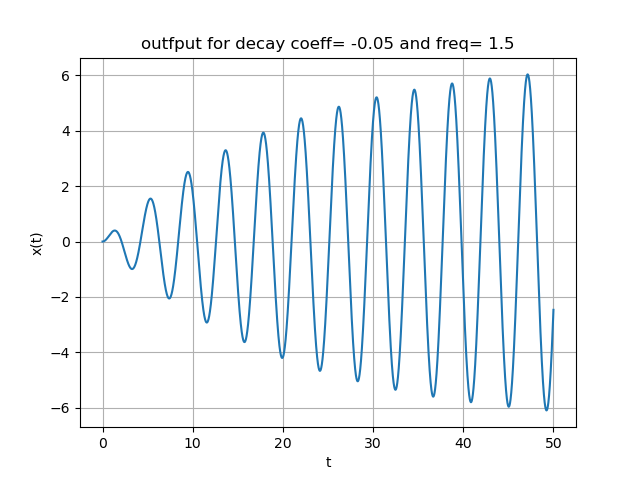
\includegraphics[scale = 1]{Figure_2.png}
    \caption{Response of a forced oscillatory system}
\end{figure}

\subsubsection{Code}
\begin{python}
#Question 2:

H2 = H_s(0.05,1.5)

t2,x2 = sp.impulse(H2,None, linspace(0,50,10000))
plot(t2,x2)
xlabel('t')
ylabel('x(t)')
title('outfput for decay coeff= -0.05 and freq= 1.5')
grid()
show()
\end{python}

\subsubsection{Observations}
We can see that Plot2 and Plot1 are very similar, but plot 2 takes a longer time to reach steady state as its decay coefficient is lower.


\subsection{Question 3: over a range of frequencies}
We now find the output if the frequency varied from 1.4 to 1.6 in increments of 0.05.

\subsubsection{Plot}
\begin{figure}[H]
    \centering
    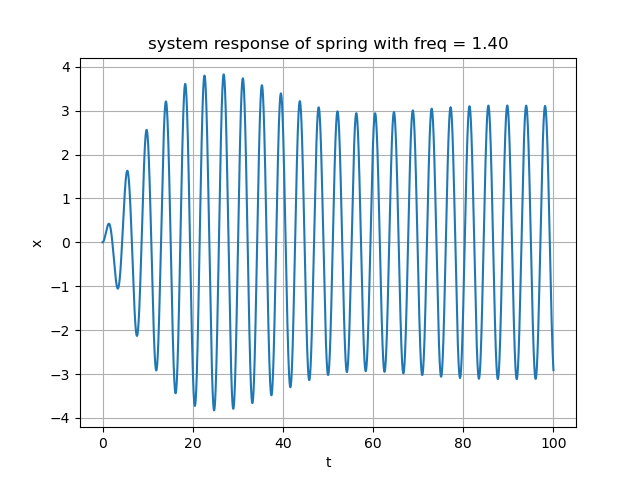
\includegraphics[scale = 1]{Figure_3.png}
    \caption{Response of a forced oscillatory system}
\end{figure}

\subsubsection{Plot}
\begin{figure}[H]
    \centering
    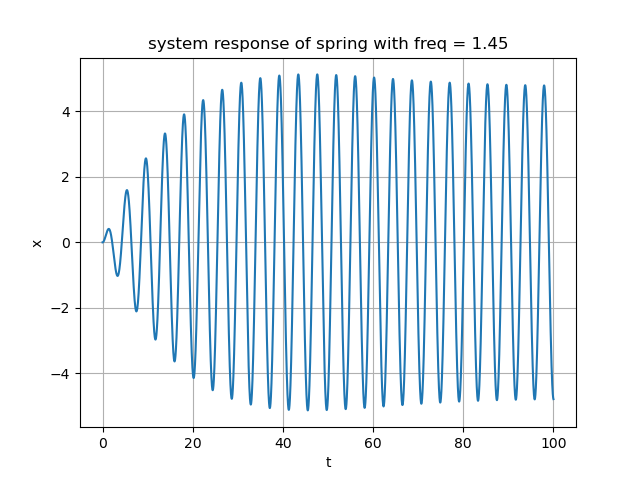
\includegraphics[scale = 1]{Figure_4.png}
    \caption{Response of a forced oscillatory system}
\end{figure}

\subsubsection{Plot}
\begin{figure}[H]
    \centering
    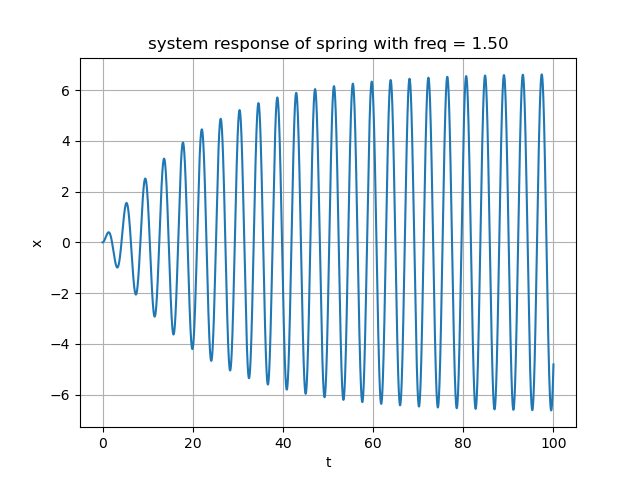
\includegraphics[scale = 1]{Figure_5.png}
    \caption{Response of a forced oscillatory system}
\end{figure}

\subsubsection{Plot}
\begin{figure}[H]
    \centering
    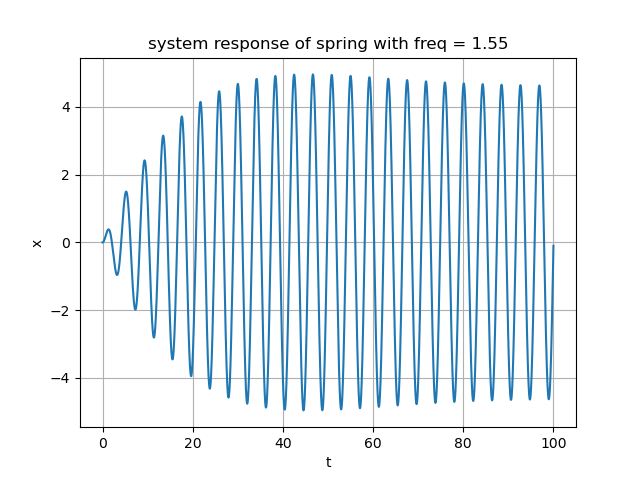
\includegraphics[scale = 1]{Figure_6.png}
    \caption{Response of a forced oscillatory system}
\end{figure}

\subsubsection{Plot}
\begin{figure}[H]
    \centering
    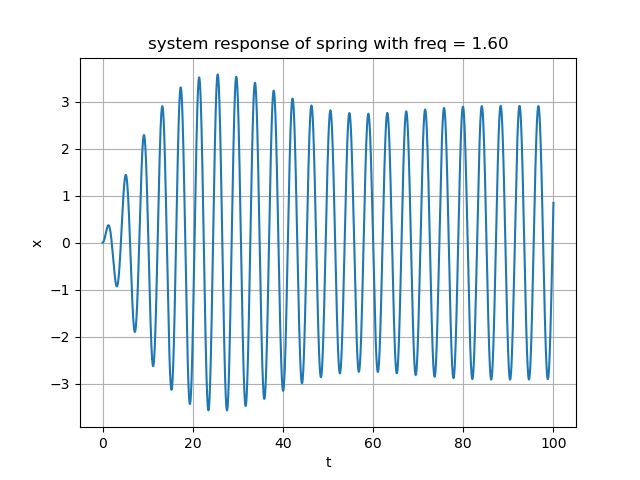
\includegraphics[scale = 1]{Figure_7.png}
    \caption{Response of a forced oscillatory system}
\end{figure}

\subsubsection{Observations and Analysis}
We can clearly see that the closer the frequency is to 1.5, the higher the amplitude at steady state. The reason for this is because the resonant frequency of the system is 1.5. (As given in the system equation).
This is the reason at frequency = 1.5, the graph is extremely smooth and has the highest amplitude at steady state.

\subsubsection{Code}
\begin{python}
#Question 3:

for i in range(5): #finding output for a range of frequencies from 1.4 to 1.6 with 0.05 increments
	f = 1.4 + i*0.05
	H = H_s(0.05,f)
	t,x = sp.impulse(H,None, linspace(0,100,10000))
	xlabel('t')
	ylabel('x')
	title('system response of spring with freq = %0.2f'%f)
	plot(t,x)
	grid()
	show()
\end{python}


\subsection{Question 4: Coupled spring problem}
The equations are:
\begin{equation}
    \"{x} + (x-y) = 0
\end{equation}
\begin{equation}
    \"{y} +2(y-x) = 0
\end{equation}
after solving, we get the fourth order equation:
\begin{equation}
    \ddddot{x} + 3\"{x} = 0
\end{equation}
with initial conditions.

on solving, we get:
\begin{equation}
    X(s) = \frac{s^2 + 2}{s^3 + 2s}
\end{equation}
\begin{equation}
    Y(s) = \frac{2}{s^3 + 2s}
\end{equation}

in time domain, for a time between 0 and 20seconds,
\subsubsection{Plot of x(t)}
\begin{figure}[H]
    \centering
    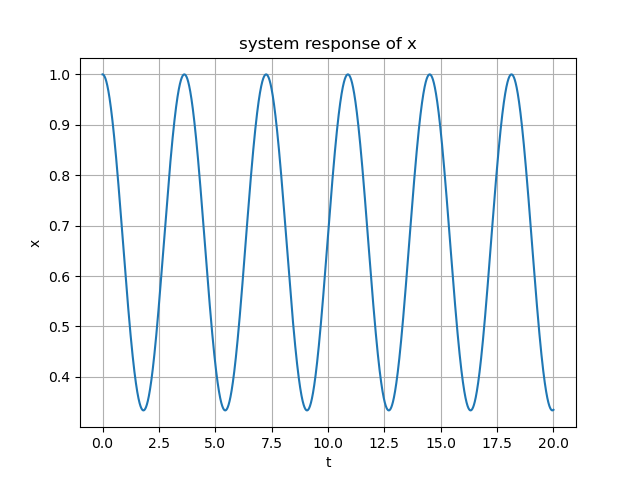
\includegraphics[scale = 1]{Figure_8.png}
    \caption{x(t)}
\end{figure}

\subsubsection{Plot of y(t)}
\begin{figure}[H]
    \centering
    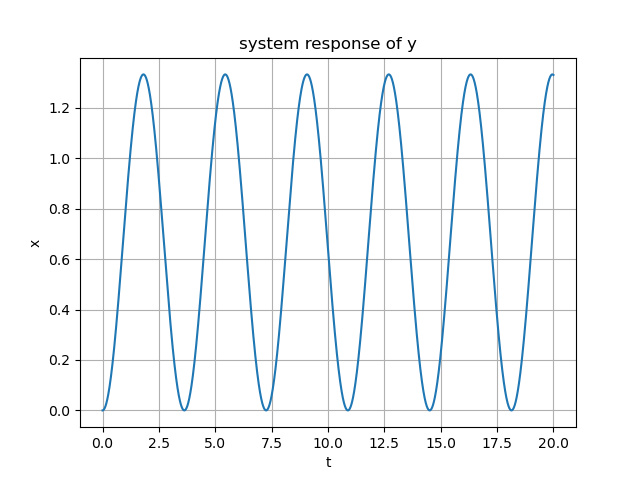
\includegraphics[scale = 1]{Figure_9.png}
    \caption{y(t)}
\end{figure}

\subsubsection{Observations}
We see that both are sinusoidal, but the amplitudes and phases of both of them are different.

\subsubsection{Code}
\begin{python}
#Question 4:

H_x = sp.lti([1,0,2],[1,0,3,0])
H_y = sp.lti([2],[1,0,3,0])

t,x = sp.impulse(H_x,None, linspace(0,20,10000))
xlabel('t')
ylabel('x')
title('system response of x')
plot(t,x)
grid()
show()

t,x = sp.impulse(H_y,None, linspace(0,20,10000))
xlabel('t')
ylabel('x')
title('system response of y')
plot(t,x)
grid()
show()
\end{python}

\subsection{Question 5: Response of the Steady State Transfer function of an RLC network}
The steady state transfer function is :
\begin{equation}
    H(s) = \frac{10^6}{s^2 + 100s + 10^6}
\end{equation}
Using H.bode(), we can plot the bode plots.

\subsubsection{Magnitude bode plot}
\begin{figure}[H]
    \centering
    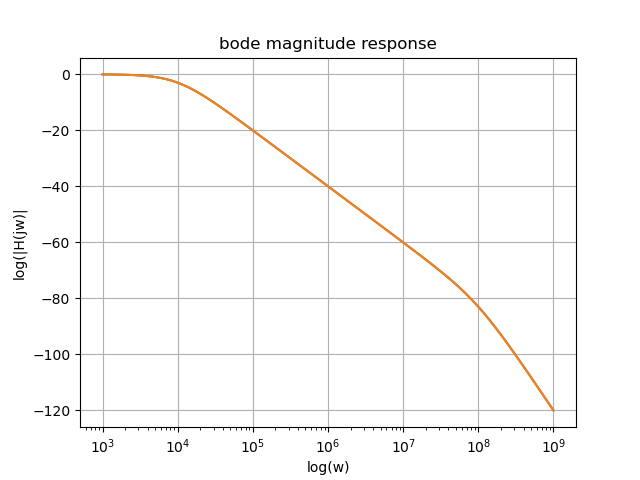
\includegraphics[scale = 1]{Figure_10.png}
    \caption{Bode magnitude plot}
\end{figure}

\subsubsection{Magnitude phase plot}
\begin{figure}[H]
    \centering
    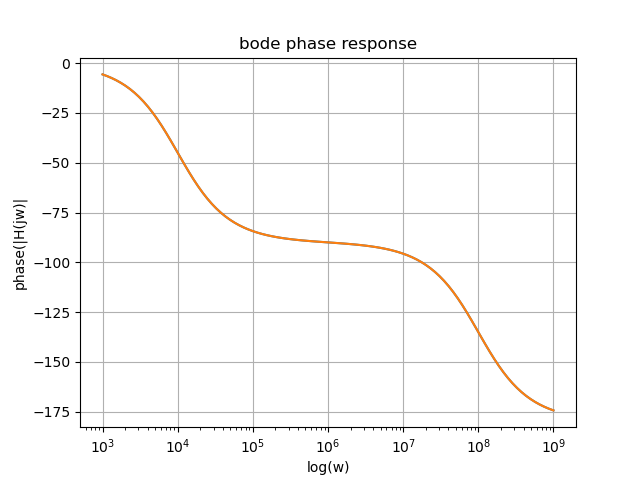
\includegraphics[scale = 1]{Figure_11.png}
    \caption{Bode Phase plot}
\end{figure}

\subsubsection{Code}
\begin{python}
#Question 5:

L = 1e-6
C = 1e-6
R = 100

H = sp.lti(1,[L*C,R*C,1]) #transfer function
w,S,phi = H.bode()
semilogx(w,S)
xlabel('log(w)')
ylabel('log(|H(jw)|')
title('bode magnitude response')
plot(w,S)
grid()
show()

semilogx(w,phi)
xlabel('log(w)')
ylabel('phase(|H(jw)|')
title('bode phase response')
plot(w,phi)
grid()
show()
\end{python}

\subsection{Question 6:}
When input is given by,
\begin{equation}
    v_i(t) = cos(10^3t)u(t) - cos(10^6t)u(t)
\end{equation}

We get the output $v_o(t)$ by finding the convolution of x(t) and $v_i(t)$,
we do this using sp.lsim method.

\subsubsection{Signal between 0 and 30$\mu$s}
\begin{figure}[H]
    \centering
    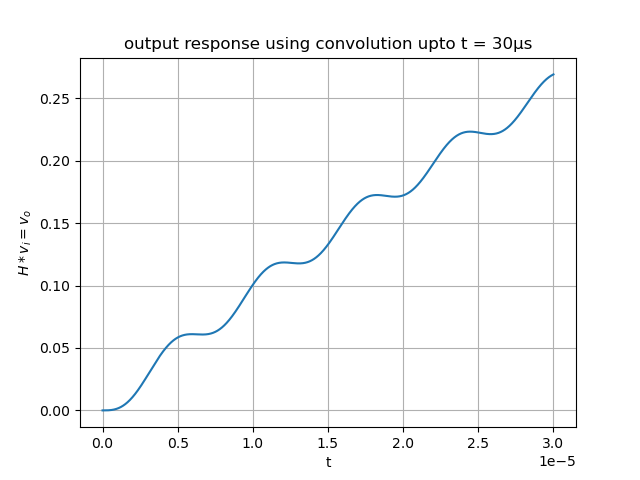
\includegraphics[scale = 1]{Figure_13.png}
\end{figure}

\subsubsection{Signal between 30ms and 32.5ms}
\begin{figure}[H]
    \centering
    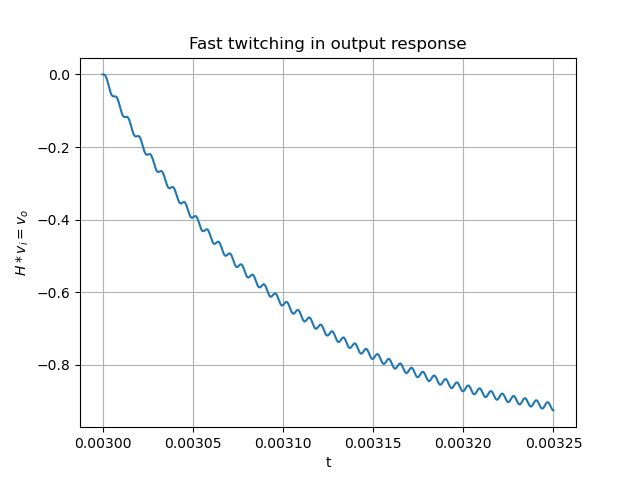
\includegraphics[scale = 1]{Figure_14.png}
\end{figure}

\subsubsection{Signal between 0 and 10ms}
\begin{figure}[H]
    \centering
    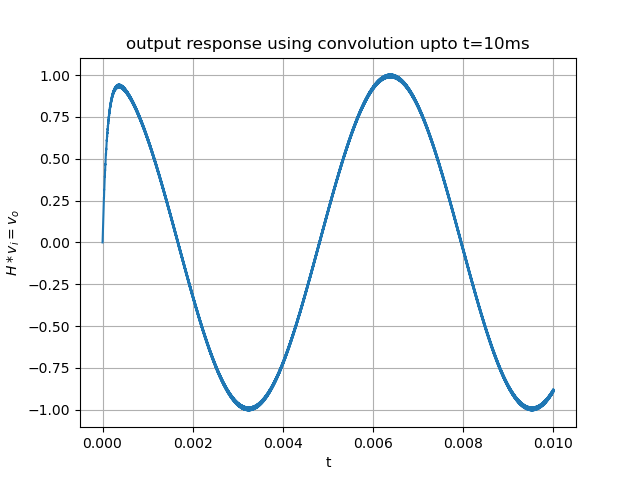
\includegraphics[scale = 1]{Figure_12.png}
\end{figure}

\subsubsection{Observations}
the reason we see a small periodic change in the output is because the original RLC circuit is a low pass filter, so it filters out the $10^6$ component of frequency. and since its not an ideal filter, this just means the magnitude of the low frequency is decreased. Hence the output consists of $10^3$ component with a small varying $10^6$ component.

\subsubsection{Code}
\begin{python}
#Question 6:

t = linspace(0,1e-2,10000)
v_i = cos(1e3*t) - cos(1e6*t)
t,y,svec = sp.lsim(H,v_i,t)
plot(t,y)
xlabel('t')
ylabel('$H * v_i = v_o$')
title('output response using convolution upto t=10ms')
grid()
show()

t = linspace(0,30*1e-6,10000)
v_i = cos(1e3*t) - cos(1e6*t)
t,y,svec = sp.lsim(H,v_i,t)
plot(t,y)
xlabel('t')
ylabel('$H * v_i = v_o$')
title('output response using convolution upto t = 30\u03BCs')
grid()
show()


t = linspace(3*1e-3,3.25*1e-3,10000)
v_i = cos(1e3*t) - cos(1e6*t)
t,y,svec = sp.lsim(H,v_i,t)
plot(t,y)
xlabel('t')
ylabel('$H * v_i = v_o$')
title('Fast twitching in output response')
grid()
show()
\end{python}

\section{Conclusions}
In this assignment, we have learnt how to use scipy.signal, a Signal analysing tool box in python. We have learnt how to find the response of a rational LTI system along with how to find the convolution of two functions in the time domain.







\end{document}
